\documentclass[11pt]{article}
\usepackage{geometry}
\usepackage{graphicx}
\usepackage{enumitem}
\usepackage{float}
\usepackage{amsmath}
\usepackage{multicol}

\geometry{a4paper, top=0.5in, bottom=0.5in, right=0.75in, left=0.75in}

\title{Lecture 1}
\author{}
\date{}

\begin{document}

\maketitle

\section{Introduction}
\begin{itemize}
    \item \textbf{Light Scattering:}  The reflection and transmission of light by a medium.
    \item \textbf{Light Interactions:}  This only happens when photon energy is higher than the energy gap of the material. This leads to the excitation of the electrons in the material.
    \item Laser light is coherent meaning there is no phase change with time.
\end{itemize}

\section{Classical Electron Oscillator Model (CEO)}
We can model the forces between nucleus and electron as a mass spring system. There is an attraction force between the electron and the nucleus. The repulsion force is the centrifugal force, so:

\begin{equation*}
    \frac{kq_1q_2}{r^2} = \frac{mv^2}{r}
\end{equation*}

\subsection{Natural Response (No External Force)}
\subsubsection{Undamped Oscillation}
\begin{align*}
    m\frac{d^2x}{dt^2} = -kx \\
    \frac{d^2x}{dt^2} + \omega_0^2 x = 0 \\
    x = A\cos(\omega_0 t + \phi)
\end{align*}
where $\omega_0 = \sqrt{\frac{k}{m}}$ is the natural frequency.

\begin{center}
    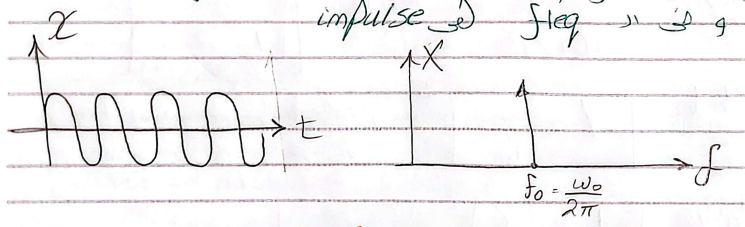
\includegraphics[scale=0.8]{1.png}
\end{center}

\begin{itemize}
    \item Since there are no losses, we get a pure sinusoidal wave in time domain or an impulse in frequency domain.
    \item Light can only interact at the resonance frequency of the material.
    \item Similar to a pendulum, energy can be calculated at the point of maximum displacement where KE = 0, given by: $E = \frac{1}{2}k_sx_{max}^2$.
\end{itemize}

\subsection{Damped Oscillation}
\begin{align*}
    m\frac{d^2x}{dt^2} = -kx - b\frac{dx}{dt} \\
    \frac{d^2x}{dt^2} + \eta\frac{dx}{dt} + \omega_0^2 x = 0 \\
    x = Ae^{-\frac{\eta}{2}t}\cos(\omega_d t + \phi)
\end{align*}
where:
\begin{itemize}
    \item $\omega_d = \sqrt{\omega_0^2 - \frac{\eta^2}{2}}$ is the damped frequency.
    \item $\eta = \frac{b}{m}$ is the damping factor.
\end{itemize}

\begin{center}
    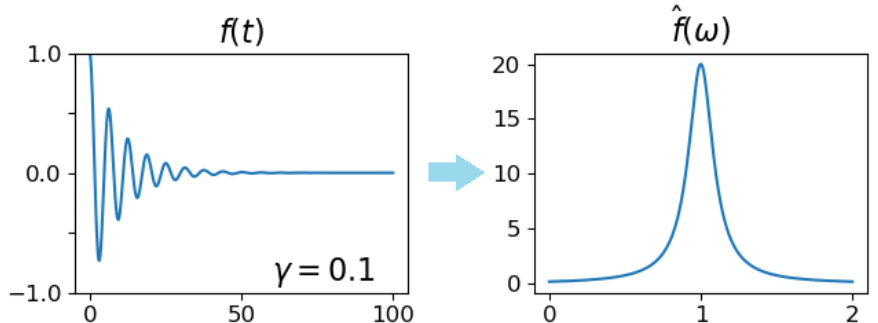
\includegraphics[scale=0.7]{2.png}
\end{center}

\begin{itemize}
    \item The presence of losses creates an underdamped time response and a broadened impulse in the frequency domain.
    \item \textbf{Why underdamped?} Since $\eta = \frac{1}{\tau}$ where $\tau$ is the electron lifetime (in nano range), while $\omega_0$ is in the Giga range, so $\omega_0 >> \frac{\eta}{2}$.
    \item Due to the broadening caused by the losses, there is a bandwidth where light can interact with the material.
    \item Assume that maximum displacement is the envelope of the damped oscillation, so:
        \begin{align*}
            x_{max} = Ae^{-\frac{\eta}{2}t} \\
            U = \frac{1}{2}k_sA^2e^{-\eta t}
        \end{align*}
\end{itemize}

\subsubsection{Losses}
\begin{itemize}
    \item \textbf{Radiation:} The accelaeration of the electron causes an electromagnetic wave to be emitted.
    \item \textbf{Collision:} The electron collides with the lattice and loses energy.
    \item The electron lifetime is the average time an electron remains in a specific energy state before transitioning to another state.
    \item Similar to time constant in an RC circuit, $e^{-\eta t} = e^{-\frac{t}{\tau}}$ 
    \item $\frac{1}{\tau} = \frac{1}{\tau_r} + \frac{1}{\tau_{nr}}$, where $\tau_r$ is the radiative lifetime and $\tau_{nr}$ is the non-radiative lifetime.
\end{itemize}

\subsection{Quantum-Mechanical Approach of Broadening}

Recall that Heisenberg's Uncertainty Principle states that we cannot know the exact energy at a specific time ($\Delta E \Delta t \geq \frac{\hbar}{2}$). This means that there is no exact energy level ($E_2 + \Delta E$) for the electron to transition to, so each electron can gain different energy and still transition. Recall that the energy of a photon is frequency dependent ($E = h \nu$), so light-matter interaction can happen at a range of frequencies (broadening). 
\pagebreak
\\
If we observe the light intensity of the source, we find a decrease in intensity due to the absorption of the material in the frequency range around resonance frequency ($\nu_0$).
\begin{center}
    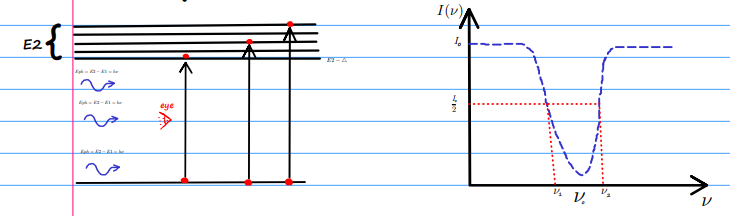
\includegraphics[width=0.9\textwidth]{6.png}
\end{center}
When an electron goes to a higher energy level, it will eventually come back to the ground state. This causes the emission of a photon with the same frequency as the absorbed photon.
\begin{center}
    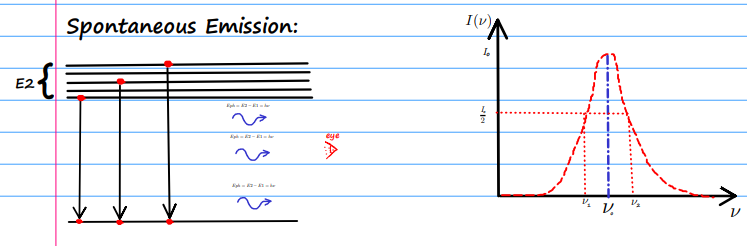
\includegraphics[width=0.9\textwidth]{7.png}
\end{center}
Note that if there was no losses, the drop and rise in intensity would be an impulse.


\subsection{Forced Response}
\textbf{Note:} We can neglect the magnetic force:
    \begin{align*}
        \frac{|F_{mag}|}{|F_{elec}|} = \frac{qvB}{qE} = \frac{vB}{E} = \frac{v}{c} << 1
    \end{align*}
Applied Sinusoidal Electric Field:
\begin{align*}
    m\frac{d^2x}{dt^2} + b\frac{dx}{dt} + k_sx = qE \\
    \frac{d^2x}{dt^2} + \eta\frac{dx}{dt} + \omega_0^2 x = \frac{qE}{m} \\
\end{align*}
Assume steady state (replace $\frac{d}{dt}$ with $j\omega$):
\begin{align*}
    -\omega^2x + j\eta\omega x + \omega_0^2 x = \frac{qE}{m} \\
    x(\omega_0^2 - \omega^2 + j\eta\omega) = \frac{qE}{m} \\
    x ((\omega_0 - \omega)(\omega_0 + \omega) + j\eta\omega) = \frac{qE}{m} \\
\end{align*}
Assume that $\omega \approx \omega_0$:
\begin{align*}
    x\left( 2\omega(\omega_0 - \omega) + j\eta\omega \right) &= \frac{qE}{m} \\
    \frac{\omega \eta}{j}x \left( \frac{2j(\omega_0 - \omega)}{\eta} - 1 \right) &= \frac{qE}{m} \\
    -\frac{\omega \eta}{j}x \left( 1 + \frac{2j(\omega - \omega_0)}{\eta} \right) &= \frac{qE}{m} \\
    x = \frac{-jqE}{m\omega\eta} \frac{1}{1 + \frac{2j(\omega - \omega_0)}{\eta}}
\end{align*}
Notes:
\begin{itemize}
    \item We want to obtain material parameters, such as relative permitivity ($\epsilon$) or susceptibility ($\chi$) to study the light-matter interaction in the material.
    \item Note that the $x$ in the dipole moment ($p=qx$) is the $\Delta x$ from equilibrium position (electron shell).
    \item Polarization is the dipole moment per unit volume ($P = N_aqx$), where $N_a$ is the number of atoms per unit volume.
    \item For linear polarization, $P = \epsilon_0\chi E$.
\end{itemize}
From polarization equations:
\begin{align*}
    P = \epsilon_0\chi E = \frac{-jN_aq^2E}{m\omega\eta} \frac{1}{1 + \frac{2j(\omega - \omega_0)}{\eta}} \\
    \chi = \frac{-jN_aq^2}{m\omega\eta\epsilon_0} \frac{1}{1 + \frac{2j(\omega - \omega_0)}{\eta}}
\end{align*}
Let $\delta = \frac{2(\omega - \omega_0)}{\eta}$:
\begin{align*}
    \chi = \frac{-jN_aq^2}{m\omega\eta\epsilon_0} \frac{1}{1 + j\delta} 
\end{align*}
Multiply by the conjugate:
\begin{align*}
    \chi = \frac{-jN_aq^2}{m\omega\eta\epsilon_0} \frac{1 - j\delta}{1 + \delta^2} \\
    \chi' = \frac{N_aq^2}{m \omega \eta \epsilon_0} \frac{-\delta}{1 + \delta^2} \\
    \chi'' = j\frac{N_aq^2}{m \omega \eta \epsilon_0} \frac{-1}{1 + \delta^2}
\end{align*}
\\
Drawing the susceptibility:
\begin{itemize}
    \item Let $\chi_0 = \frac{N_aq^2}{m \omega \eta \epsilon_0}$.
    \item $\delta = \frac{2(\omega - \omega_0)}{\eta}$
\end{itemize}
\underline{Max \& Min for $\chi'$:}
\begin{align*}
    \frac{d \chi'}{d \delta} = \chi_0 \frac{1-\delta^2}{(1+\delta^2)^2} = 0 \rightarrow \delta = \pm1
\end{align*}
\begin{align*}
    \omega = \omega_0 \pm \frac{\eta}{2}
\end{align*}
\underline{Max $\chi'$:}
\begin{align*}
    \frac{d \chi''}{d \delta} = \chi_0 \frac{-2\delta}{(1+\delta^2)^2} = 0 \rightarrow \delta = 0
\end{align*}
\begin{align*}
    \omega = \omega_0
\end{align*}
\begin{center}
    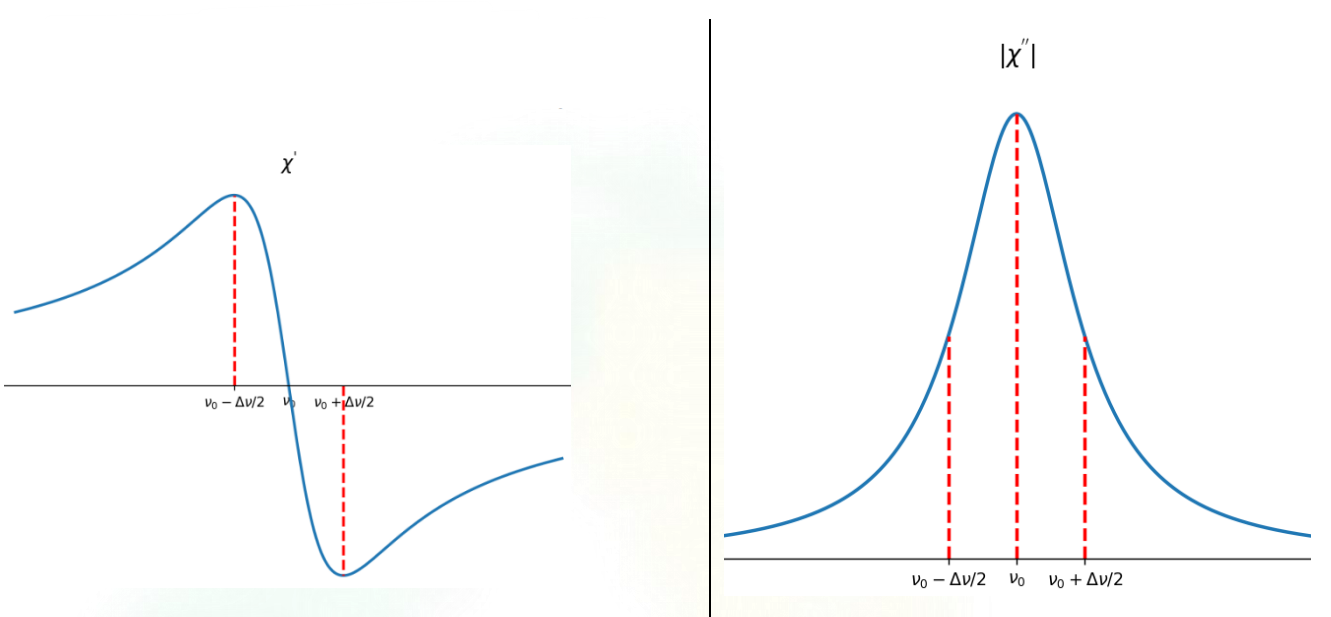
\includegraphics[scale=0.5]{3.png}
\end{center}
From previous equations, we can draw the relative permitivity using the susceptibility:
\[
    \epsilon_r = 1 + \chi = 1 + \chi' + j\chi''
\]
\begin{center}
    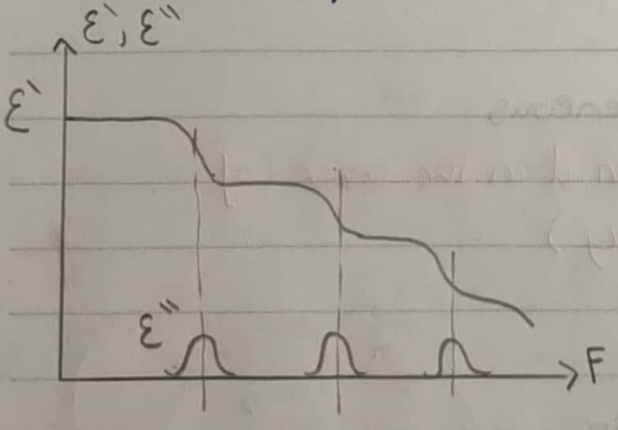
\includegraphics[scale=0.5]{5.png}
\end{center}
Proof that $\chi''$ leads to attenuation:
\begin{align*}
    k = k_0\sqrt{\epsilon_r} = k_0\sqrt{1 + \chi' + \chi''} \\
    = k_0\sqrt{(1+\chi') \left( 1+j\frac{\chi''}{1+\chi'} \right)} \\
    = k_0\sqrt{1+\chi'}\sqrt{1+j\frac{\chi''}{1+\chi'}} \\
\end{align*}
Note that $\sqrt{1+\chi'} = \sqrt{\epsilon'} = n$, so:
\[k_0n \sqrt{1+j\frac{\chi''}{n^2}} \approx k_0n \left(1 + j \frac{\chi''}{2n^2}\right)\]
Therefore:
\begin{itemize}
    \item lossless propagation constant: $k_0n$
    \item lossy propagation constant ($\gamma$): $\gamma = k_0\frac{\chi''}{2n}$ (Always negative in classical model)
\end{itemize}
Recall that wave propagation has $e^{jkx}$ term, so the real term in k will be the phase term, while the imaginary term will be the attenuation term.

\end{document}